% Options for packages loaded elsewhere
% Options for packages loaded elsewhere
\PassOptionsToPackage{unicode}{hyperref}
\PassOptionsToPackage{hyphens}{url}
\PassOptionsToPackage{dvipsnames,svgnames,x11names}{xcolor}
%
\documentclass[
  authoryear,
  preprint]{elsarticle}
\usepackage{xcolor}
\usepackage{amsmath,amssymb}
\setcounter{secnumdepth}{5}
\usepackage{iftex}
\ifPDFTeX
  \usepackage[T1]{fontenc}
  \usepackage[utf8]{inputenc}
  \usepackage{textcomp} % provide euro and other symbols
\else % if luatex or xetex
  \usepackage{unicode-math} % this also loads fontspec
  \defaultfontfeatures{Scale=MatchLowercase}
  \defaultfontfeatures[\rmfamily]{Ligatures=TeX,Scale=1}
\fi
\usepackage{lmodern}
\ifPDFTeX\else
  % xetex/luatex font selection
\fi
% Use upquote if available, for straight quotes in verbatim environments
\IfFileExists{upquote.sty}{\usepackage{upquote}}{}
\IfFileExists{microtype.sty}{% use microtype if available
  \usepackage[]{microtype}
  \UseMicrotypeSet[protrusion]{basicmath} % disable protrusion for tt fonts
}{}
\makeatletter
\@ifundefined{KOMAClassName}{% if non-KOMA class
  \IfFileExists{parskip.sty}{%
    \usepackage{parskip}
  }{% else
    \setlength{\parindent}{0pt}
    \setlength{\parskip}{6pt plus 2pt minus 1pt}}
}{% if KOMA class
  \KOMAoptions{parskip=half}}
\makeatother
% Make \paragraph and \subparagraph free-standing
\makeatletter
\ifx\paragraph\undefined\else
  \let\oldparagraph\paragraph
  \renewcommand{\paragraph}{
    \@ifstar
      \xxxParagraphStar
      \xxxParagraphNoStar
  }
  \newcommand{\xxxParagraphStar}[1]{\oldparagraph*{#1}\mbox{}}
  \newcommand{\xxxParagraphNoStar}[1]{\oldparagraph{#1}\mbox{}}
\fi
\ifx\subparagraph\undefined\else
  \let\oldsubparagraph\subparagraph
  \renewcommand{\subparagraph}{
    \@ifstar
      \xxxSubParagraphStar
      \xxxSubParagraphNoStar
  }
  \newcommand{\xxxSubParagraphStar}[1]{\oldsubparagraph*{#1}\mbox{}}
  \newcommand{\xxxSubParagraphNoStar}[1]{\oldsubparagraph{#1}\mbox{}}
\fi
\makeatother

\usepackage{color}
\usepackage{fancyvrb}
\newcommand{\VerbBar}{|}
\newcommand{\VERB}{\Verb[commandchars=\\\{\}]}
\DefineVerbatimEnvironment{Highlighting}{Verbatim}{commandchars=\\\{\}}
% Add ',fontsize=\small' for more characters per line
\usepackage{framed}
\definecolor{shadecolor}{RGB}{241,243,245}
\newenvironment{Shaded}{\begin{snugshade}}{\end{snugshade}}
\newcommand{\AlertTok}[1]{\textcolor[rgb]{0.68,0.00,0.00}{#1}}
\newcommand{\AnnotationTok}[1]{\textcolor[rgb]{0.37,0.37,0.37}{#1}}
\newcommand{\AttributeTok}[1]{\textcolor[rgb]{0.40,0.45,0.13}{#1}}
\newcommand{\BaseNTok}[1]{\textcolor[rgb]{0.68,0.00,0.00}{#1}}
\newcommand{\BuiltInTok}[1]{\textcolor[rgb]{0.00,0.23,0.31}{#1}}
\newcommand{\CharTok}[1]{\textcolor[rgb]{0.13,0.47,0.30}{#1}}
\newcommand{\CommentTok}[1]{\textcolor[rgb]{0.37,0.37,0.37}{#1}}
\newcommand{\CommentVarTok}[1]{\textcolor[rgb]{0.37,0.37,0.37}{\textit{#1}}}
\newcommand{\ConstantTok}[1]{\textcolor[rgb]{0.56,0.35,0.01}{#1}}
\newcommand{\ControlFlowTok}[1]{\textcolor[rgb]{0.00,0.23,0.31}{\textbf{#1}}}
\newcommand{\DataTypeTok}[1]{\textcolor[rgb]{0.68,0.00,0.00}{#1}}
\newcommand{\DecValTok}[1]{\textcolor[rgb]{0.68,0.00,0.00}{#1}}
\newcommand{\DocumentationTok}[1]{\textcolor[rgb]{0.37,0.37,0.37}{\textit{#1}}}
\newcommand{\ErrorTok}[1]{\textcolor[rgb]{0.68,0.00,0.00}{#1}}
\newcommand{\ExtensionTok}[1]{\textcolor[rgb]{0.00,0.23,0.31}{#1}}
\newcommand{\FloatTok}[1]{\textcolor[rgb]{0.68,0.00,0.00}{#1}}
\newcommand{\FunctionTok}[1]{\textcolor[rgb]{0.28,0.35,0.67}{#1}}
\newcommand{\ImportTok}[1]{\textcolor[rgb]{0.00,0.46,0.62}{#1}}
\newcommand{\InformationTok}[1]{\textcolor[rgb]{0.37,0.37,0.37}{#1}}
\newcommand{\KeywordTok}[1]{\textcolor[rgb]{0.00,0.23,0.31}{\textbf{#1}}}
\newcommand{\NormalTok}[1]{\textcolor[rgb]{0.00,0.23,0.31}{#1}}
\newcommand{\OperatorTok}[1]{\textcolor[rgb]{0.37,0.37,0.37}{#1}}
\newcommand{\OtherTok}[1]{\textcolor[rgb]{0.00,0.23,0.31}{#1}}
\newcommand{\PreprocessorTok}[1]{\textcolor[rgb]{0.68,0.00,0.00}{#1}}
\newcommand{\RegionMarkerTok}[1]{\textcolor[rgb]{0.00,0.23,0.31}{#1}}
\newcommand{\SpecialCharTok}[1]{\textcolor[rgb]{0.37,0.37,0.37}{#1}}
\newcommand{\SpecialStringTok}[1]{\textcolor[rgb]{0.13,0.47,0.30}{#1}}
\newcommand{\StringTok}[1]{\textcolor[rgb]{0.13,0.47,0.30}{#1}}
\newcommand{\VariableTok}[1]{\textcolor[rgb]{0.07,0.07,0.07}{#1}}
\newcommand{\VerbatimStringTok}[1]{\textcolor[rgb]{0.13,0.47,0.30}{#1}}
\newcommand{\WarningTok}[1]{\textcolor[rgb]{0.37,0.37,0.37}{\textit{#1}}}

\usepackage{longtable,booktabs,array}
\usepackage{calc} % for calculating minipage widths
% Correct order of tables after \paragraph or \subparagraph
\usepackage{etoolbox}
\makeatletter
\patchcmd\longtable{\par}{\if@noskipsec\mbox{}\fi\par}{}{}
\makeatother
% Allow footnotes in longtable head/foot
\IfFileExists{footnotehyper.sty}{\usepackage{footnotehyper}}{\usepackage{footnote}}
\makesavenoteenv{longtable}
\usepackage{graphicx}
\makeatletter
\newsavebox\pandoc@box
\newcommand*\pandocbounded[1]{% scales image to fit in text height/width
  \sbox\pandoc@box{#1}%
  \Gscale@div\@tempa{\textheight}{\dimexpr\ht\pandoc@box+\dp\pandoc@box\relax}%
  \Gscale@div\@tempb{\linewidth}{\wd\pandoc@box}%
  \ifdim\@tempb\p@<\@tempa\p@\let\@tempa\@tempb\fi% select the smaller of both
  \ifdim\@tempa\p@<\p@\scalebox{\@tempa}{\usebox\pandoc@box}%
  \else\usebox{\pandoc@box}%
  \fi%
}
% Set default figure placement to htbp
\def\fps@figure{htbp}
\makeatother





\setlength{\emergencystretch}{3em} % prevent overfull lines

\providecommand{\tightlist}{%
  \setlength{\itemsep}{0pt}\setlength{\parskip}{0pt}}



 
\usepackage[]{natbib}
\bibliographystyle{elsarticle-harv}


\makeatletter
\@ifpackageloaded{caption}{}{\usepackage{caption}}
\AtBeginDocument{%
\ifdefined\contentsname
  \renewcommand*\contentsname{Table of contents}
\else
  \newcommand\contentsname{Table of contents}
\fi
\ifdefined\listfigurename
  \renewcommand*\listfigurename{List of Figures}
\else
  \newcommand\listfigurename{List of Figures}
\fi
\ifdefined\listtablename
  \renewcommand*\listtablename{List of Tables}
\else
  \newcommand\listtablename{List of Tables}
\fi
\ifdefined\figurename
  \renewcommand*\figurename{Figure}
\else
  \newcommand\figurename{Figure}
\fi
\ifdefined\tablename
  \renewcommand*\tablename{Table}
\else
  \newcommand\tablename{Table}
\fi
}
\@ifpackageloaded{float}{}{\usepackage{float}}
\floatstyle{ruled}
\@ifundefined{c@chapter}{\newfloat{codelisting}{h}{lop}}{\newfloat{codelisting}{h}{lop}[chapter]}
\floatname{codelisting}{Listing}
\newcommand*\listoflistings{\listof{codelisting}{List of Listings}}
\makeatother
\makeatletter
\makeatother
\makeatletter
\@ifpackageloaded{caption}{}{\usepackage{caption}}
\@ifpackageloaded{subcaption}{}{\usepackage{subcaption}}
\makeatother
\journal{Journal Name}
\usepackage{bookmark}
\IfFileExists{xurl.sty}{\usepackage{xurl}}{} % add URL line breaks if available
\urlstyle{same}
\hypersetup{
  pdftitle={Stroop Task Replication Study},
  pdfauthor={Christina Fan; Daniella Christina Pereira Cisorio; Alexia Nijgorodov; Diya Renjan},
  pdfkeywords={Stroop task, cognitive interference, cognitive
control, automaticity, congruency, reaction
time, accuracy, replication},
  colorlinks=true,
  linkcolor={blue},
  filecolor={Maroon},
  citecolor={Blue},
  urlcolor={Blue},
  pdfcreator={LaTeX via pandoc}}


\setlength{\parindent}{6pt}
\begin{document}

\begin{frontmatter}
\title{Stroop Task Replication Study}
\author[1]{Christina Fan%
%
}

\author[1]{Daniella Christina Pereira Cisorio%
%
}

\author[1]{Alexia Nijgorodov%
%
}

\author[1]{Diya Renjan%
%
}


\affiliation[1]{organization={University of Waterloo, Department of
Psychology},,postcodesep={}}

\cortext[cor1]{Corresponding author}




        
\begin{abstract}
This study aimed to replicate the Stroop effect, which predicts slower
reaction times and lower accuracy for incongruent compared to congruent
colour-word stimuli. Fifteen undergraduate participants completed a
computerized Stroop task, and reaction time and accuracy were analyzed
using two-way repeated measures ANOVAs. Contrary to our hypothesis, no
significant main effect of congruency was found on reaction time or
accuracy. The lack of significant findings may be due to methodological
limitations, including a small sample size, fewer trials, and the
presence of extreme outliers. Future research should increase
statistical power by using a larger number of trials and participants,
and apply stricter data screening procedures.
\end{abstract}





\begin{keyword}
    Stroop task \sep cognitive interference \sep cognitive
control \sep automaticity \sep congruency \sep reaction
time \sep accuracy \sep 
    replication
\end{keyword}
\end{frontmatter}
    

\section{Introduction}\label{introduction}

The Stroop effect is one of the most well-known phenomena in cognitive
psychology. First demonstrated by John Ridley Stroop in 1935, the effect
refers to the cognitive interference that occurs when the brain is
presented with two conflicting pieces of information at the same time.
In the conventional Stroop task, participants are shown colour words
printed in different ink colours and are asked to name the colour of the
word, ignoring the word itself. The task consists of two conditions. In
congruent trials, the word and ink colour match (e.g the word ``RED''
written in red). In incongruent trials, the word and ink colour do not
match (e.g.~the word ``RED'' written in blue). The task measures
reaction time and accuracy as objective indicators of cognitive
interference experienced during incongruent trials. The Stroop task is
often used to measure attention, processing speed, and cognitive
control.

\citet{Stroop1935} originally found that participants were significantly
slower and less accurate when naming colours on incongruent trials
compared to congruent ones. This effect has been replicated across
hundreds of studies, making it a very reliable finding
\citep{MacLeod1991}. It was also found that with practice, interference
decreases over time, though it never fully disappears, suggesting the
effect reflects automatic reading and limits in cognitive control.
Several theories have been proposed to explain why the Stroop effect
occurs. The relative speed of processing theory suggests that the brain
processes written words faster than colours, so the word meaning reaches
the response stage first and interferes with the colour naming
\citep{MacLeod1991}. The automaticity theory proposes that reading is
such a highly practiced process that it occurs automatically, which
interferes with the slower, more deliberate process of colour naming
which draws more heavily on attentional resources \citep{MacLeod1991}.
While these theories explain parts of the effect, there is no single
universally accepted explanation for the Stroop effect.

This present study aimed to replicate the Stroop effect. Based on
previous research, we hypothesized that participants would show slower
reaction times and lower accuracy on incongruent trials compared to
congruent trials.

\section{Methods}\label{methods}

This study replicated the Stroop Effect by implementing the word-color
visualizations on a computer screen. We wrote an experimental program in
PsychoPy, an open-source software library written in Python, that
delievered the experiment.

\subsection{Participants}\label{participants}

Fifteen participants in the age range of 19-25 were recruited from an
undergraduate upper-year psychology seminar course at the University of
Waterloo. Each participant completed the Stroop Task on one of the
researcher's computer.

\subsection{Experimental Task Design}\label{experimental-task-design}

Participants are introduced to the experiment with instructions
describing the experiment protocol. After reading, participants are
instructed to press the spacebar to proceed to the first trial of the
experiment. There are a total of 3 trials, with 10 words being shown to
participants in each trial. Each word is shown on the screen for 500 ms
before disappearing, and participants are required to press a key to
indicate the color of the word. The next word will not appear until
participants give a response to the current word.
Figure~\ref{fig-experiment_visual} shows an illustration of the
experiment protocol.

\begin{figure}[H]

\centering{

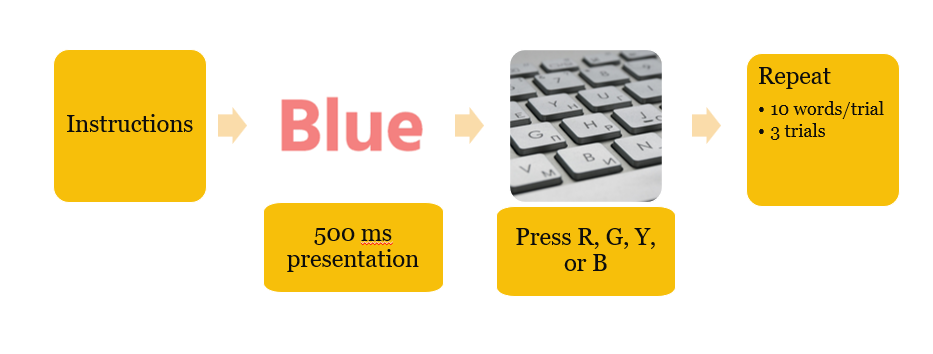
\includegraphics[width=0.6\linewidth,height=\textheight,keepaspectratio]{article_images/task_flowchart.png}

}

\caption{\label{fig-experiment_visual}Experiment Protocol Flowchart}

\end{figure}%

The program randomly generates color words from the list: red, green,
blue, yellow and the color of those words are also randomly selected
among those colors. Thus, the chances of a word presentation being
congruent or incongruent are random. The keys ``r'', ``g'',``b'',``y''
are assigned to the respective colors red, green, blue, yellow for
participants to give their response when reporting the color of the
word. Participants are able to exit the experiment at any time by
pressing the ``Esc'' key.

\subsection{Data Processing and
Analysis}\label{data-processing-and-analysis}

During the experiment, the congruency of each word is recorded, and the
participant's reaction time (the time in between stimulus presentation
and keyboard response), and accuracy of response are recorded. These
results are stored in a CSV file generated for each participant.

Two 2-way repeated measures ANOVA tests were performed examining the
main effects of trial and congruency on reaction time and accuracy.
Interactions effects between trial and congruency were considered on
reaction time and accuracy as well.

\section{Results}\label{results}

All of the data from the study was included in the results, including
outliers such as participants with extremely high reaction times or
extremely poor accuracy.

\subsection{Reaction Time - Overall vs Congruent vs
Incongruent}\label{reaction-time---overall-vs-congruent-vs-incongruent}

\subsubsection{Daniella in-line}\label{daniella-in-line}

The overall results including both congruent and incongruent words were
analyzed first. The mean reaction time across all trials was about
\texttt{python\ mean\_rt} seconds. Shown in Figure 1, reaction time
decreased sharply between Trial 1 (M = 1.63s) and Trial 2 (M = 1.10s)
before evening out in Trial 3 (M = 1.09s). Figure 2 demonstrates the
average reaction times of congruent and incongruent words. The mean
reaction time for congruent words across all trials was about 1.19
seconds while the mean reaction time for incongruent words across all
trials was about 1.28 seconds. Trial 1 went against the hypothesis as
the mean reaction time for congruent words (M = 1.63s) was higher than
that of incongruent words (M = 1.56s). However, this was not the same
for trials 2 and 3. In trial 2, the mean reaction time for congruent
words (M = 0.92s) ended up lower than incongruent words (M = 1.16s).
Trial 3 followed this same trend with congruent words (M = 1.02) being
lower than incongruent words (M = 1.14s). However, unlike the overall
results the mean reaction time for congruent words rose slightly from
trial 2 to trial 3.

\subsection{Accuracy - Overall vs Congruent vs
Incongruent}\label{accuracy---overall-vs-congruent-vs-incongruent}

\subsubsection{Daniella in-line}\label{daniella-in-line-1}

The overall results including both congruent and incongruent words were
analyzed first, with the mean accuracy across all trials coming out to
about \texttt{python\ mean\_accuracy}. Shown in Figure 3, accuracy in
Trial 1 starts off fairly low (M = 81.8\%) and rises steadily through
Trial 2 (M = 87.5\%) and reaches a peak at Trial 3 (M = 90.0\%). When
compared to the average accuracy based on congruency, the trend shifts
away from a steady rise. The mean accuracy for congruent words across
all trials was about 92.0\%, where incongruent words ended up with a
mean accuracy of about 81.3\%. Figure 4 demonstrates the mean accuracy
based on each trial. Trial 1 started with a large gap between congruent
words (M = 91.7\%) and incongruent words (M = 76.5\%). Despite congruent
accuracy remaining higher than incongruent accuracy, Trial 2 saw a drop
in congruent accuracy (M = 87.5\%) and a rise in incongruent accuracy (M
= 82.9\%). However, Trial 3 saw a rise in both congruent accuracy (M =
96.9\%) and incongruent accuracy (M = 84.6\%). Although there was a rise
in both congruent and incongruent accuracy, congruent words remained
higher than incongruent words through all trials.

\subsection{Interaction between congruency and trial on reaction
time}\label{interaction-between-congruency-and-trial-on-reaction-time}

\subsection{Christina anova}\label{christina-anova}

In order to analyze the effects of trial and congruency on reaction
time, a 2-way repeated measures ANOVA was conducted. Demonstrated in
Table 1, the results yielded insignificant effects. There was no
significant main effect found of congruency (F(1, 13)=0.07, p =0.799),
meaning there was not a noticeable difference of reaction time between
congruent and incongruent conditions. Trial came just short of reaching
a significant main effect (F(2, 28) = 3.36, p = 0.049). Although trial
did not reach statistical significance, this suggests there is a
possible trend in reaction time among trials. In addition, the
interaction between congruency and trial showed no significance (F(2,
28) = 0.29, p = 0.752), meaning there is no significant effect of
congruency on reaction time across time. Despite the potential trend of
the trial condition, the results of this ANOVA found no significant main
effects of congruency on reaction time.

\subsection{Interaction between congruency and trial on
accuracy}\label{interaction-between-congruency-and-trial-on-accuracy}

\subsection{hopefully daniella can adapt from above to here if it
works}\label{hopefully-daniella-can-adapt-from-above-to-here-if-it-works}

In order to analyze the effect of trial and congruency on accuracy, a
2-way repeated measures ANOVA was conducted. Demonstrated in Table 2,
similar to the results of the first ANOVA conducted, the results yielded
insignificant effects. There was no significant main effect found of
congruency (F(1, 13) = 5.69, p = 0.033), meaning there was no
significant difference of accuracy between congruent and incongruent
trials. There was no significant main effect found of trial (F(2, 28) =
0.48, p = 0.621), meaning accuracy did not noticeably differ between
trials. Unlike the previous ANOVA where trial had a slight trend, this
one did not provide a trend of trial. Additionally, the interaction
between congruency and trial showed no significance (F(2, 28) = 1.86, p
= 0.175), meaning there is no significant effect of congruency on
accuracy across time. Like the results of the previous ANOVA, there were
no significant main effects of congruency on accuracy.

\begin{figure}[H]

\centering{

\pandocbounded{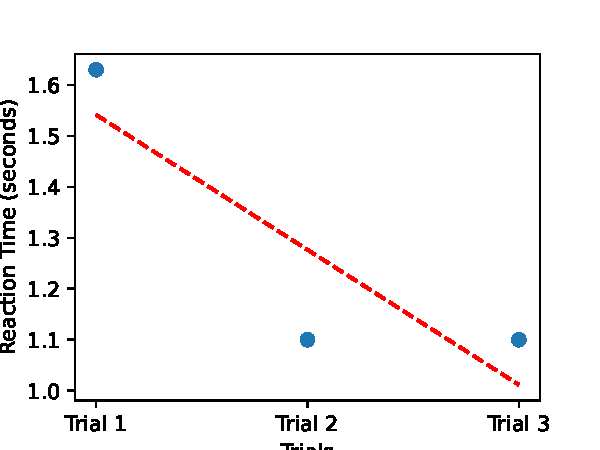
\includegraphics[keepaspectratio]{stroop_article_files/figure-pdf/fig-rt-overall-1.pdf}}

}

\caption{\label{fig-rt-overall}Changes in Mean Reaction Time Across
Trials}

\end{figure}%

\begin{verbatim}
([<matplotlib.axis.XTick object at 0x745ca407b070>, <matplotlib.axis.XTick object at 0x745c9f6bd360>, <matplotlib.axis.XTick object at 0x745c9f6fa4d0>], [Text(0, 0, 'Trial 1'), Text(1, 0, 'Trial 2'), Text(2, 0, 'Trial 3')])
\end{verbatim}

\begin{figure}[H]

\centering{

\pandocbounded{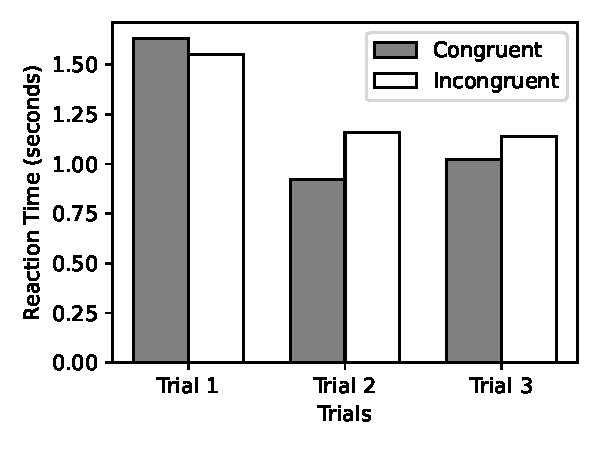
\includegraphics[keepaspectratio]{stroop_article_files/figure-pdf/fig-rt-congruency-3.pdf}}

}

\caption{\label{fig-rt-congruency}Effects of Congruency on Reaction
Time}

\end{figure}%

\subsection{Accuracy - Overall vs Congruent vs
Incongruent}\label{accuracy---overall-vs-congruent-vs-incongruent-1}

\subsection{Daniella in-line}\label{daniella-in-line-2}

The overall results including both congruent and incongruent words were
analyzed first, with the mean accuracy across all trials coming out to
about 86.4\%. Shown in Figure~\ref{fig-acc-overall}, accuracy in Trial 1
starts off fairly low (M = 81.8\%) and rises steadily through Trial 2 (M
= 87.5\%) and reaches a peak at Trial 3 (M = 90.0\%). When compared to
the average accuracy based on congruency, the trend shifts away from a
steady rise. The mean accuracy for congruent words across all trials was
about 92.0\%, where incongruent words ended up with a mean accuracy of
about 81.3\%. Figure~\ref{fig-acc-congruency} demonstrates the mean
accuracy based on each trial. Trial 1 started with a large gap between
congruent words (M = 91.7\%) and incongruent words (M = 76.5\%). Despite
congruent accuracy remaining higher than incongruent accuracy, Trial 2
saw a drop in congruent accuracy (M = 87.5\%) and a rise in incongruent
accuracy (M = 82.9\%). However, Trial 3 saw a rise in both congruent
accuracy (M = 96.9\%) and incongruent accuracy (M = 84.6\%). Although
there was a rise in both congruent and incongruent accuracy, congruent
words remained higher than incongruent words through all trials.

\begin{figure}[H]

\centering{

\pandocbounded{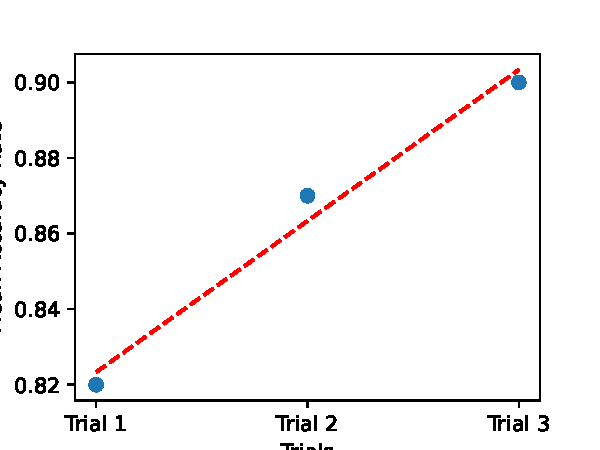
\includegraphics[keepaspectratio]{stroop_article_files/figure-pdf/fig-acc-overall-5.pdf}}

}

\caption{\label{fig-acc-overall}Changes in Mean Accuracy Rates Across
Trials}

\end{figure}%

\begin{verbatim}
([<matplotlib.axis.XTick object at 0x745c9f630430>, <matplotlib.axis.XTick object at 0x745c9f631480>, <matplotlib.axis.XTick object at 0x745c9f5bc460>], [Text(0, 0, 'Trial 1'), Text(1, 0, 'Trial 2'), Text(2, 0, 'Trial 3')])
\end{verbatim}

\begin{verbatim}
(0.0, 1.3)
\end{verbatim}

\begin{figure}[H]

\centering{

\pandocbounded{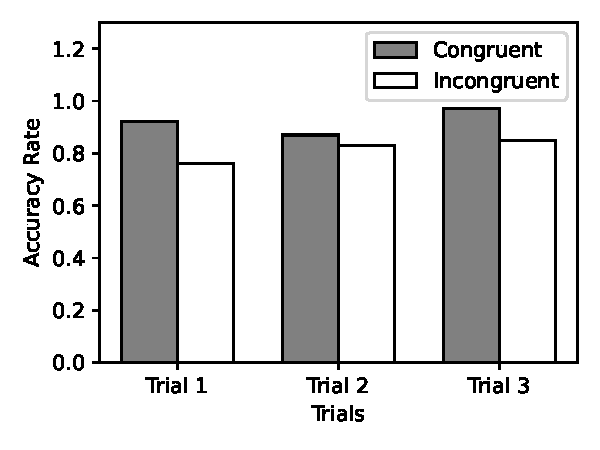
\includegraphics[keepaspectratio]{stroop_article_files/figure-pdf/fig-acc-congruency-7.pdf}}

}

\caption{\label{fig-acc-congruency}Effects of Congruency on Accuracy}

\end{figure}%

\subsection{Interaction between congruency and trial on reaction
time}\label{interaction-between-congruency-and-trial-on-reaction-time-1}

\subsection{hopefully daniella can adapt from above to here if it
works}\label{hopefully-daniella-can-adapt-from-above-to-here-if-it-works-1}

In order to analyze the effects of trial and congruency on reaction
time, a 2-way repeated measures ANOVA was conducted. Demonstrated in
Table~\ref{tbl-rt-anova}, the results yielded insignificant effects.
There was no significant main effect found of congruency (F(1,15) =
0.200, p = 0.661), meaning there was not a noticeable difference of
reaction time between congruent and incongruent conditions. Trial came
just short of reaching a significant main effect (F(2,30) = 3.178, p =
0.056). Although trial did not reach statistical significance, this
suggests there is a possible trend in reaction time among trials. In
addition, the interaction between congruency and trial showed no
significance (F(2,30) = 0.280, p = 0.758), meaning there is no
significant effect of congruency on reaction time across time. Despite
the potential trend of the trial condition, the results of this ANOVA
found no significant main effects of congruency on reaction time.

\subsection{christina anova table}\label{christina-anova-table}

\begin{verbatim}
         Effect DFn DFd    F     p
1         Match   1  13 0.07 0.799
2         Trial   2  28 3.36 0.049
3 Match × Trial   2  28 0.29 0.752
\end{verbatim}

\begin{table}

\caption{\label{tbl-rt-anova}Repeated Measures ANOVA for Reaction Time}

\centering{

\begin{verbatim}
                Effect  Sum of Squares  df  Mean Square      F      p
0           Congruency           0.204   1        0.204  0.200  0.661
1   Error (Congruency)          15.344  15        1.023    NaN    NaN
2                Trial           6.035   2        3.017  3.178  0.056
3        Error (Trial)          28.486  30        0.950    NaN    NaN
4   Congruency × Trial           0.400   2        0.200  0.280  0.758
5  Error (Interaction)          21.441  30        0.715    NaN    NaN
\end{verbatim}

}

\end{table}%

\subsection{Interaction between congruency and trial on
accuracy}\label{interaction-between-congruency-and-trial-on-accuracy-1}

\subsection{hopefully daniella can adapt from above TABLE to here if it
works}\label{hopefully-daniella-can-adapt-from-above-table-to-here-if-it-works}

In order to analyze the effect of trial and congruency on accuracy, a
2-way repeated measures ANOVA was conducted. Demonstrated in
Table~\ref{tbl-acc-anova}, similar to the results of the first ANOVA
conducted, the results yielded insignificant effects. There was no
significant main effect found of congruency (F(1,15) = 2.479, p =
0.136), meaning there was no significant difference of accuracy between
congruent and incongruent trials. There was no significant main effect
found of trial (F(2,30) = 1.128, p = 0.337), meaning accuracy did not
noticeably differ between trials. Unlike the previous ANOVA where trial
had a slight trend, this one did not provide a trend of trial.
Additionally, the interaction between congruency and trial showed no
significance (F(2,30) = 0.488, p = 0.619), meaning there is no
significant effect of congruency on accuracy across time. Like the
results of the previous ANOVA, there were no significant main effects of
congruency on accuracy.

\begin{verbatim}
         Effect DFn DFd    F     p
1         Match   1  13 5.69 0.033
2         Trial   2  28 0.48 0.621
3 Match × Trial   2  28 1.86 0.175
\end{verbatim}

\begin{table}

\caption{\label{tbl-acc-anova}Repeated Measures ANOVA for Accuracy}

\centering{

\begin{verbatim}
                Effect  Sum of Squares  df  Mean Square      F      p
0           Congruency           0.275   1        0.275  2.479  0.136
1   Error (Congruency)           1.666  15        0.111    NaN    NaN
2                Trial           0.083   2        0.041  1.128  0.337
3        Error (Trial)           1.099  30        0.037    NaN    NaN
4   Congruency × Trial           0.048   2        0.024  0.488  0.619
5  Error (Interaction)           1.469  30        0.049    NaN    NaN
\end{verbatim}

}

\end{table}%

\begin{Shaded}
\begin{Highlighting}[]
\ImportTok{import}\NormalTok{ pandas }\ImportTok{as}\NormalTok{ pd}

\NormalTok{data }\OperatorTok{=}\NormalTok{ pd.DataFrame(\{}
    \StringTok{"reaction\_time"}\NormalTok{: [}\FloatTok{0.681}\NormalTok{, }\FloatTok{0.524}\NormalTok{, }\FloatTok{0.628}\NormalTok{, }\FloatTok{0.769}\NormalTok{, }\FloatTok{0.599}\NormalTok{, }\FloatTok{0.659}\NormalTok{, }\FloatTok{0.610}\NormalTok{, }\FloatTok{0.675}\NormalTok{, }\FloatTok{0.588}\NormalTok{, }\FloatTok{0.678}\NormalTok{, }\FloatTok{0.545}\NormalTok{, }\FloatTok{0.641}\NormalTok{, }\FloatTok{0.576}\NormalTok{, }\FloatTok{0.561}\NormalTok{, }\FloatTok{0.616}\NormalTok{, }\FloatTok{0.580}\NormalTok{, }\FloatTok{0.670}\NormalTok{, }\FloatTok{0.721}\NormalTok{, }\FloatTok{0.801}\NormalTok{, }\FloatTok{0.572}\NormalTok{, }\FloatTok{0.549}\NormalTok{, }\FloatTok{0.743}\NormalTok{, }\FloatTok{0.534}\NormalTok{, }\FloatTok{0.607}\NormalTok{, }\FloatTok{0.603}\NormalTok{, }\FloatTok{0.561}\NormalTok{, }\FloatTok{1.203}\NormalTok{, }\FloatTok{0.577}\NormalTok{, }\FloatTok{0.562}\NormalTok{, }\FloatTok{0.574}\NormalTok{, }\FloatTok{1.231}\NormalTok{, }\FloatTok{1.144}\NormalTok{, }\FloatTok{1.289}\NormalTok{, }\FloatTok{1.160}\NormalTok{, }\FloatTok{1.278}\NormalTok{, }\FloatTok{1.419}\NormalTok{, }\FloatTok{1.241}\NormalTok{, }\FloatTok{2.117}\NormalTok{, }\FloatTok{1.300}\NormalTok{, }\FloatTok{1.519}\NormalTok{, }\FloatTok{1.179}\NormalTok{, }\FloatTok{1.201}\NormalTok{, }\FloatTok{1.641}\NormalTok{, }\FloatTok{1.209}\NormalTok{, }\FloatTok{1.463}\NormalTok{, }\FloatTok{1.917}\NormalTok{, }\FloatTok{1.089}\NormalTok{, }\FloatTok{1.009}\NormalTok{, }\FloatTok{1.075}\NormalTok{, }\FloatTok{1.258}\NormalTok{, }\FloatTok{1.241}\NormalTok{, }\FloatTok{1.302}\NormalTok{, }\FloatTok{1.187}\NormalTok{, }\FloatTok{1.263}\NormalTok{, }\FloatTok{1.493}\NormalTok{, }\FloatTok{1.171}\NormalTok{, }\FloatTok{1.243}\NormalTok{, }\FloatTok{1.349}\NormalTok{, }\FloatTok{2.632}\NormalTok{, }\FloatTok{5.719}\NormalTok{, }\FloatTok{1.430}\NormalTok{, }\FloatTok{13.240}\NormalTok{, }\FloatTok{2.506}\NormalTok{, }\FloatTok{1.480}\NormalTok{, }\FloatTok{13.747}\NormalTok{, }\FloatTok{1.602}\NormalTok{, }\FloatTok{2.473}\NormalTok{, }\FloatTok{0.864}\NormalTok{, }\FloatTok{4.781}\NormalTok{, }\FloatTok{1.184}\NormalTok{, }\FloatTok{1.185}\NormalTok{, }\FloatTok{3.710}\NormalTok{, }\FloatTok{1.517}\NormalTok{, }\FloatTok{1.431}\NormalTok{, }\FloatTok{1.274}\NormalTok{, }\FloatTok{1.523}\NormalTok{, }\FloatTok{1.145}\NormalTok{, }\FloatTok{1.182}\NormalTok{, }\FloatTok{1.794}\NormalTok{, }\FloatTok{1.066}\NormalTok{, }\FloatTok{1.231}\NormalTok{, }\FloatTok{0.970}\NormalTok{, }\FloatTok{0.740}\NormalTok{, }\FloatTok{0.820}\NormalTok{, }\FloatTok{0.906}\NormalTok{, }\FloatTok{0.775}\NormalTok{, }\FloatTok{0.841}\NormalTok{, }\FloatTok{1.447}\NormalTok{, }\FloatTok{0.716}\NormalTok{, }\FloatTok{0.839}\NormalTok{, }\FloatTok{0.992}\NormalTok{, }\FloatTok{0.549}\NormalTok{, }\FloatTok{1.048}\NormalTok{, }\FloatTok{0.718}\NormalTok{, }\FloatTok{0.726}\NormalTok{, }\FloatTok{1.225}\NormalTok{, }\FloatTok{0.915}\NormalTok{, }\FloatTok{0.761}\NormalTok{, }\FloatTok{0.779}\NormalTok{, }\FloatTok{0.705}\NormalTok{, }\FloatTok{0.703}\NormalTok{, }\FloatTok{0.753}\NormalTok{, }\FloatTok{0.763}\NormalTok{, }\FloatTok{0.796}\NormalTok{, }\FloatTok{0.708}\NormalTok{, }\FloatTok{0.870}\NormalTok{, }\FloatTok{1.080}\NormalTok{, }\FloatTok{0.842}\NormalTok{, }\FloatTok{0.847}\NormalTok{, }\FloatTok{1.066}\NormalTok{, }\FloatTok{0.698}\NormalTok{, }\FloatTok{0.787}\NormalTok{, }\FloatTok{0.689}\NormalTok{, }\FloatTok{0.753}\NormalTok{, }\FloatTok{0.716}\NormalTok{, }\FloatTok{0.822}\NormalTok{, }\FloatTok{0.730}\NormalTok{, }\FloatTok{0.770}\NormalTok{, }\FloatTok{0.835}\NormalTok{, }\FloatTok{1.102}\NormalTok{, }\FloatTok{1.015}\NormalTok{, }\FloatTok{0.920}\NormalTok{, }\FloatTok{1.192}\NormalTok{, }\FloatTok{0.839}\NormalTok{, }\FloatTok{0.717}\NormalTok{, }\FloatTok{1.244}\NormalTok{, }\FloatTok{1.029}\NormalTok{, }\FloatTok{1.358}\NormalTok{, }\FloatTok{1.244}\NormalTok{, }\FloatTok{0.976}\NormalTok{, }\FloatTok{0.894}\NormalTok{, }\FloatTok{0.866}\NormalTok{, }\FloatTok{0.842}\NormalTok{, }\FloatTok{0.831}\NormalTok{, }\FloatTok{0.584}\NormalTok{, }\FloatTok{0.688}\NormalTok{, }\FloatTok{1.370}\NormalTok{, }\FloatTok{0.846}\NormalTok{, }\FloatTok{0.611}\NormalTok{, }\FloatTok{0.645}\NormalTok{, }\FloatTok{0.777}\NormalTok{, }\FloatTok{1.001}\NormalTok{, }\FloatTok{0.756}\NormalTok{, }\FloatTok{0.782}\NormalTok{, }\FloatTok{1.039}\NormalTok{, }\FloatTok{1.008}\NormalTok{, }\FloatTok{0.845}\NormalTok{, }\FloatTok{0.918}\NormalTok{, }\FloatTok{0.764}\NormalTok{, }\FloatTok{0.664}\NormalTok{, }\FloatTok{0.803}\NormalTok{, }\FloatTok{0.839}\NormalTok{, }\FloatTok{0.664}\NormalTok{, }\FloatTok{0.645}\NormalTok{, }\FloatTok{0.831}\NormalTok{, }\FloatTok{0.624}\NormalTok{, }\FloatTok{0.727}\NormalTok{, }\FloatTok{0.684}\NormalTok{, }\FloatTok{0.704}\NormalTok{, }\FloatTok{0.593}\NormalTok{, }\FloatTok{0.557}\NormalTok{, }\FloatTok{0.583}\NormalTok{, }\FloatTok{0.632}\NormalTok{, }\FloatTok{0.603}\NormalTok{, }\FloatTok{0.563}\NormalTok{, }\FloatTok{0.766}\NormalTok{, }\FloatTok{9.214}\NormalTok{, }\FloatTok{0.751}\NormalTok{, }\FloatTok{0.613}\NormalTok{, }\FloatTok{0.643}\NormalTok{, }\FloatTok{1.820}\NormalTok{, }\FloatTok{1.196}\NormalTok{, }\FloatTok{1.316}\NormalTok{, }\FloatTok{1.128}\NormalTok{, }\FloatTok{1.015}\NormalTok{, }\FloatTok{1.010}\NormalTok{, }\FloatTok{0.785}\NormalTok{, }\FloatTok{0.900}\NormalTok{, }\FloatTok{0.712}\NormalTok{, }\FloatTok{0.898}\NormalTok{, }\FloatTok{1.037}\NormalTok{, }\FloatTok{1.427}\NormalTok{, }\FloatTok{0.807}\NormalTok{, }\FloatTok{0.725}\NormalTok{, }\FloatTok{1.742}\NormalTok{, }\FloatTok{0.847}\NormalTok{, }\FloatTok{0.807}\NormalTok{, }\FloatTok{0.925}\NormalTok{, }\FloatTok{0.770}\NormalTok{, }\FloatTok{1.284}\NormalTok{, }\FloatTok{0.932}\NormalTok{, }\FloatTok{1.032}\NormalTok{, }\FloatTok{0.742}\NormalTok{, }\FloatTok{1.179}\NormalTok{, }\FloatTok{0.952}\NormalTok{, }\FloatTok{0.792}\NormalTok{, }\FloatTok{0.835}\NormalTok{, }\FloatTok{0.900}\NormalTok{, }\FloatTok{0.849}\NormalTok{, }\FloatTok{0.810}\NormalTok{, }\FloatTok{0.819}\NormalTok{, }\FloatTok{0.737}\NormalTok{, }\FloatTok{0.685}\NormalTok{, }\FloatTok{0.642}\NormalTok{, }\FloatTok{0.522}\NormalTok{, }\FloatTok{0.543}\NormalTok{, }\FloatTok{0.699}\NormalTok{, }\FloatTok{0.706}\NormalTok{, }\FloatTok{1.548}\NormalTok{, }\FloatTok{0.965}\NormalTok{, }\FloatTok{1.521}\NormalTok{, }\FloatTok{1.206}\NormalTok{, }\FloatTok{1.081}\NormalTok{, }\FloatTok{2.590}\NormalTok{, }\FloatTok{1.021}\NormalTok{, }\FloatTok{0.972}\NormalTok{, }\FloatTok{0.990}\NormalTok{, }\FloatTok{0.856}\NormalTok{, }\FloatTok{0.996}\NormalTok{, }\FloatTok{1.090}\NormalTok{, }\FloatTok{0.922}\NormalTok{, }\FloatTok{0.780}\NormalTok{, }\FloatTok{0.933}\NormalTok{, }\FloatTok{1.015}\NormalTok{, }\FloatTok{1.193}\NormalTok{, }\FloatTok{0.937}\NormalTok{, }\FloatTok{0.817}\NormalTok{, }\FloatTok{0.984}\NormalTok{, }\FloatTok{0.965}\NormalTok{, }\FloatTok{0.862}\NormalTok{, }\FloatTok{0.757}\NormalTok{, }\FloatTok{0.835}\NormalTok{, }\FloatTok{0.759}\NormalTok{, }\FloatTok{0.799}\NormalTok{, }\FloatTok{1.019}\NormalTok{, }\FloatTok{0.768}\NormalTok{, }\FloatTok{1.190}\NormalTok{, }\FloatTok{1.112}\NormalTok{, }\FloatTok{0.937}\NormalTok{, }\FloatTok{0.963}\NormalTok{, }\FloatTok{1.677}\NormalTok{, }\FloatTok{1.377}\NormalTok{, }\FloatTok{1.346}\NormalTok{, }\FloatTok{1.572}\NormalTok{, }\FloatTok{1.425}\NormalTok{, }\FloatTok{1.448}\NormalTok{, }\FloatTok{1.450}\NormalTok{, }\FloatTok{1.309}\NormalTok{, }\FloatTok{1.679}\NormalTok{, }\FloatTok{1.736}\NormalTok{, }\FloatTok{1.175}\NormalTok{, }\FloatTok{0.966}\NormalTok{, }\FloatTok{1.016}\NormalTok{, }\FloatTok{1.118}\NormalTok{, }\FloatTok{1.731}\NormalTok{, }\FloatTok{1.463}\NormalTok{, }\FloatTok{1.233}\NormalTok{, }\FloatTok{1.458}\NormalTok{, }\FloatTok{1.445}\NormalTok{, }\FloatTok{1.135}\NormalTok{, }\FloatTok{1.015}\NormalTok{, }\FloatTok{1.430}\NormalTok{, }\FloatTok{1.540}\NormalTok{, }\FloatTok{0.863}\NormalTok{, }\FloatTok{0.991}\NormalTok{, }\FloatTok{0.784}\NormalTok{, }\FloatTok{1.070}\NormalTok{, }\FloatTok{1.125}\NormalTok{, }\FloatTok{0.968}\NormalTok{, }\FloatTok{1.594}\NormalTok{, }\FloatTok{1.088}\NormalTok{, }\FloatTok{1.069}\NormalTok{, }\FloatTok{0.690}\NormalTok{, }\FloatTok{19.209}\NormalTok{, }\FloatTok{0.988}\NormalTok{, }\FloatTok{0.756}\NormalTok{, }\FloatTok{1.378}\NormalTok{, }\FloatTok{0.922}\NormalTok{, }\FloatTok{0.707}\NormalTok{, }\FloatTok{0.799}\NormalTok{, }\FloatTok{0.762}\NormalTok{, }\FloatTok{0.750}\NormalTok{, }\FloatTok{0.904}\NormalTok{, }\FloatTok{3.663}\NormalTok{, }\FloatTok{0.750}\NormalTok{, }\FloatTok{0.886}\NormalTok{, }\FloatTok{0.595}\NormalTok{, }\FloatTok{0.859}\NormalTok{, }\FloatTok{0.605}\NormalTok{, }\FloatTok{1.037}\NormalTok{, }\FloatTok{0.785}\NormalTok{, }\FloatTok{0.743}\NormalTok{, }\FloatTok{0.690}\NormalTok{, }\FloatTok{0.805}\NormalTok{, }\FloatTok{0.606}\NormalTok{, }\FloatTok{0.603}\NormalTok{, }\FloatTok{0.902}\NormalTok{, }\FloatTok{0.736}\NormalTok{, }\FloatTok{0.624}\NormalTok{, }\FloatTok{0.837}\NormalTok{, }\FloatTok{1.656}\NormalTok{, }\FloatTok{1.607}\NormalTok{, }\FloatTok{1.953}\NormalTok{, }\FloatTok{1.445}\NormalTok{, }\FloatTok{3.871}\NormalTok{, }\FloatTok{1.588}\NormalTok{, }\FloatTok{1.754}\NormalTok{, }\FloatTok{1.168}\NormalTok{, }\FloatTok{1.771}\NormalTok{, }\FloatTok{1.876}\NormalTok{, }\FloatTok{1.014}\NormalTok{, }\FloatTok{1.068}\NormalTok{, }\FloatTok{1.180}\NormalTok{, }\FloatTok{0.967}\NormalTok{, }\FloatTok{1.034}\NormalTok{, }\FloatTok{1.223}\NormalTok{, }\FloatTok{2.154}\NormalTok{, }\FloatTok{3.485}\NormalTok{, }\FloatTok{1.761}\NormalTok{, }\FloatTok{3.024}\NormalTok{, }\FloatTok{1.033}\NormalTok{, }\FloatTok{2.738}\NormalTok{, }\FloatTok{1.085}\NormalTok{, }\FloatTok{1.052}\NormalTok{, }\FloatTok{1.168}\NormalTok{, }\FloatTok{1.092}\NormalTok{, }\FloatTok{1.421}\NormalTok{, }\FloatTok{1.584}\NormalTok{, }\FloatTok{2.055}\NormalTok{, }\FloatTok{1.491}\NormalTok{, }\FloatTok{0.734}\NormalTok{, }\FloatTok{0.843}\NormalTok{, }\FloatTok{0.874}\NormalTok{, }\FloatTok{0.914}\NormalTok{, }\FloatTok{0.945}\NormalTok{, }\FloatTok{0.826}\NormalTok{, }\FloatTok{0.833}\NormalTok{, }\FloatTok{0.782}\NormalTok{, }\FloatTok{0.850}\NormalTok{, }\FloatTok{0.789}\NormalTok{, }\FloatTok{0.737}\NormalTok{, }\FloatTok{0.878}\NormalTok{, }\FloatTok{0.849}\NormalTok{, }\FloatTok{0.777}\NormalTok{, }\FloatTok{0.839}\NormalTok{, }\FloatTok{0.987}\NormalTok{, }\FloatTok{0.853}\NormalTok{, }\FloatTok{0.866}\NormalTok{, }\FloatTok{0.920}\NormalTok{, }\FloatTok{0.758}\NormalTok{, }\FloatTok{0.796}\NormalTok{, }\FloatTok{0.807}\NormalTok{, }\FloatTok{0.728}\NormalTok{, }\FloatTok{0.825}\NormalTok{, }\FloatTok{0.704}\NormalTok{, }\FloatTok{0.842}\NormalTok{, }\FloatTok{0.705}\NormalTok{, }\FloatTok{0.770}\NormalTok{, }\FloatTok{0.758}\NormalTok{, }\FloatTok{1.340}\NormalTok{, }\FloatTok{1.681}\NormalTok{, }\FloatTok{1.149}\NormalTok{, }\FloatTok{1.278}\NormalTok{, }\FloatTok{1.258}\NormalTok{, }\FloatTok{1.391}\NormalTok{, }\FloatTok{0.935}\NormalTok{, }\FloatTok{1.428}\NormalTok{, }\FloatTok{1.039}\NormalTok{, }\FloatTok{0.984}\NormalTok{, }\FloatTok{0.922}\NormalTok{, }\FloatTok{1.211}\NormalTok{, }\FloatTok{1.053}\NormalTok{, }\FloatTok{0.801}\NormalTok{, }\FloatTok{0.854}\NormalTok{, }\FloatTok{1.041}\NormalTok{, }\FloatTok{1.058}\NormalTok{, }\FloatTok{0.912}\NormalTok{, }\FloatTok{1.001}\NormalTok{, }\FloatTok{1.121}\NormalTok{, }\FloatTok{1.018}\NormalTok{, }\FloatTok{1.025}\NormalTok{, }\FloatTok{15.257}\NormalTok{, }\FloatTok{0.936}\NormalTok{, }\FloatTok{0.697}\NormalTok{, }\FloatTok{0.692}\NormalTok{, }\FloatTok{0.899}\NormalTok{, }\FloatTok{0.814}\NormalTok{, }\FloatTok{1.139}\NormalTok{, }\FloatTok{0.928}\NormalTok{, }\FloatTok{1.116}\NormalTok{, }\FloatTok{14.691}\NormalTok{, }\FloatTok{3.276}\NormalTok{, }\FloatTok{0.880}\NormalTok{, }\FloatTok{1.964}\NormalTok{, }\FloatTok{1.139}\NormalTok{, }\FloatTok{1.466}\NormalTok{, }\FloatTok{1.089}\NormalTok{, }\FloatTok{1.024}\NormalTok{, }\FloatTok{1.294}\NormalTok{, }\FloatTok{1.288}\NormalTok{, }\FloatTok{1.008}\NormalTok{, }\FloatTok{1.695}\NormalTok{, }\FloatTok{0.951}\NormalTok{, }\FloatTok{1.016}\NormalTok{, }\FloatTok{1.389}\NormalTok{, }\FloatTok{1.136}\NormalTok{, }\FloatTok{0.932}\NormalTok{, }\FloatTok{1.171}\NormalTok{, }\FloatTok{0.966}\NormalTok{, }\FloatTok{1.368}\NormalTok{, }\FloatTok{1.036}\NormalTok{, }\FloatTok{0.996}\NormalTok{, }\FloatTok{0.822}\NormalTok{, }\FloatTok{0.934}\NormalTok{, }\FloatTok{0.834}\NormalTok{, }\FloatTok{1.292}\NormalTok{, }\FloatTok{0.909}\NormalTok{, }\FloatTok{0.963}\NormalTok{, }\FloatTok{0.991}\NormalTok{, }\FloatTok{1.116}\NormalTok{, }\FloatTok{1.358}\NormalTok{, }\FloatTok{1.409}\NormalTok{, }\FloatTok{1.787}\NormalTok{, }\FloatTok{1.685}\NormalTok{, }\FloatTok{1.220}\NormalTok{, }\FloatTok{1.561}\NormalTok{, }\FloatTok{1.367}\NormalTok{, }\FloatTok{0.711}\NormalTok{, }\FloatTok{1.464}\NormalTok{, }\FloatTok{1.970}\NormalTok{, }\FloatTok{1.108}\NormalTok{, }\FloatTok{1.161}\NormalTok{, }\FloatTok{1.117}\NormalTok{, }\FloatTok{1.229}\NormalTok{, }\FloatTok{1.031}\NormalTok{, }\FloatTok{1.377}\NormalTok{, }\FloatTok{2.021}\NormalTok{, }\FloatTok{1.394}\NormalTok{, }\FloatTok{1.232}\NormalTok{, }\FloatTok{0.595}\NormalTok{, }\FloatTok{0.905}\NormalTok{, }\FloatTok{1.505}\NormalTok{, }\FloatTok{0.858}\NormalTok{, }\FloatTok{0.789}\NormalTok{, }\FloatTok{1.917}\NormalTok{, }\FloatTok{0.686}\NormalTok{, }\FloatTok{0.804}\NormalTok{, }\FloatTok{0.761}\NormalTok{, }\FloatTok{0.733}\NormalTok{, }\FloatTok{1.614}\NormalTok{, }\FloatTok{1.102}\NormalTok{, }\FloatTok{1.099}\NormalTok{, }\FloatTok{0.864}\NormalTok{, }\FloatTok{1.180}\NormalTok{, }\FloatTok{17.071}\NormalTok{, }\FloatTok{0.743}\NormalTok{, }\FloatTok{0.674}\NormalTok{, }\FloatTok{0.535}\NormalTok{, }\FloatTok{0.805}\NormalTok{, }\FloatTok{0.755}\NormalTok{, }\FloatTok{0.705}\NormalTok{, }\FloatTok{2.476}\NormalTok{, }\FloatTok{0.663}\NormalTok{, }\FloatTok{0.549}\NormalTok{, }\FloatTok{0.536}\NormalTok{, }\FloatTok{0.546}\NormalTok{, }\FloatTok{0.757}\NormalTok{, }\FloatTok{0.678}\NormalTok{, }\FloatTok{0.699}\NormalTok{, }\FloatTok{0.543}\NormalTok{, }\FloatTok{2.352}\NormalTok{, }\FloatTok{0.566}\NormalTok{, }\FloatTok{1.946}\NormalTok{, }\FloatTok{0.526}\NormalTok{, }\FloatTok{0.745}\NormalTok{, }\FloatTok{0.658}\NormalTok{, }\FloatTok{0.608}\NormalTok{, }\FloatTok{2.898}\NormalTok{, }\FloatTok{0.514}\NormalTok{, }\FloatTok{0.569}\NormalTok{]}
\NormalTok{\})}

\NormalTok{mean\_rt }\OperatorTok{=}\NormalTok{ data[}\StringTok{"reaction\_time"}\NormalTok{].mean()}
\BuiltInTok{print}\NormalTok{(mean\_rt)}
\end{Highlighting}
\end{Shaded}

\begin{verbatim}
1.2776375000000002
\end{verbatim}

\begin{Shaded}
\begin{Highlighting}[]
\ImportTok{import}\NormalTok{ pandas }\ImportTok{as}\NormalTok{ pd}

\NormalTok{data }\OperatorTok{=}\NormalTok{ pd.DataFrame(\{}
    \StringTok{"accuracy"}\NormalTok{: [}\DecValTok{1}\NormalTok{, }\DecValTok{1}\NormalTok{, }\DecValTok{1}\NormalTok{, }\DecValTok{0}\NormalTok{, }\DecValTok{0}\NormalTok{, }\DecValTok{0}\NormalTok{, }\DecValTok{0}\NormalTok{, }\DecValTok{0}\NormalTok{, }\DecValTok{1}\NormalTok{, }\DecValTok{0}\NormalTok{, }\DecValTok{0}\NormalTok{, }\DecValTok{0}\NormalTok{, }\DecValTok{0}\NormalTok{, }\DecValTok{0}\NormalTok{, }\DecValTok{1}\NormalTok{, }\DecValTok{0}\NormalTok{, }\DecValTok{0}\NormalTok{, }\DecValTok{1}\NormalTok{, }\DecValTok{0}\NormalTok{, }\DecValTok{1}\NormalTok{, }\DecValTok{0}\NormalTok{, }\DecValTok{0}\NormalTok{, }\DecValTok{0}\NormalTok{, }\DecValTok{0}\NormalTok{, }\DecValTok{1}\NormalTok{, }\DecValTok{1}\NormalTok{, }\DecValTok{1}\NormalTok{, }\DecValTok{1}\NormalTok{, }\DecValTok{1}\NormalTok{, }\DecValTok{1}\NormalTok{, }\DecValTok{1}\NormalTok{, }\DecValTok{1}\NormalTok{, }\DecValTok{1}\NormalTok{, }\DecValTok{1}\NormalTok{, }\DecValTok{1}\NormalTok{, }\DecValTok{1}\NormalTok{, }\DecValTok{1}\NormalTok{, }\DecValTok{1}\NormalTok{, }\DecValTok{1}\NormalTok{, }\DecValTok{0}\NormalTok{, }\DecValTok{1}\NormalTok{, }\DecValTok{0}\NormalTok{, }\DecValTok{1}\NormalTok{, }\DecValTok{1}\NormalTok{, }\DecValTok{1}\NormalTok{, }\DecValTok{1}\NormalTok{, }\DecValTok{1}\NormalTok{, }\DecValTok{1}\NormalTok{, }\DecValTok{1}\NormalTok{, }\DecValTok{1}\NormalTok{, }\DecValTok{1}\NormalTok{, }\DecValTok{1}\NormalTok{, }\DecValTok{1}\NormalTok{, }\DecValTok{1}\NormalTok{, }\DecValTok{1}\NormalTok{, }\DecValTok{1}\NormalTok{, }\DecValTok{1}\NormalTok{, }\DecValTok{1}\NormalTok{, }\DecValTok{1}\NormalTok{, }\DecValTok{1}\NormalTok{, }\DecValTok{0}\NormalTok{, }\DecValTok{0}\NormalTok{, }\DecValTok{1}\NormalTok{, }\DecValTok{1}\NormalTok{, }\DecValTok{1}\NormalTok{, }\DecValTok{1}\NormalTok{, }\DecValTok{0}\NormalTok{, }\DecValTok{1}\NormalTok{, }\DecValTok{0}\NormalTok{, }\DecValTok{1}\NormalTok{, }\DecValTok{1}\NormalTok{, }\DecValTok{1}\NormalTok{, }\DecValTok{1}\NormalTok{, }\DecValTok{1}\NormalTok{, }\DecValTok{1}\NormalTok{, }\DecValTok{1}\NormalTok{, }\DecValTok{1}\NormalTok{, }\DecValTok{1}\NormalTok{, }\DecValTok{1}\NormalTok{, }\DecValTok{1}\NormalTok{, }\DecValTok{1}\NormalTok{, }\DecValTok{1}\NormalTok{, }\DecValTok{1}\NormalTok{, }\DecValTok{1}\NormalTok{, }\DecValTok{1}\NormalTok{, }\DecValTok{1}\NormalTok{, }\DecValTok{1}\NormalTok{, }\DecValTok{1}\NormalTok{, }\DecValTok{1}\NormalTok{, }\DecValTok{1}\NormalTok{, }\DecValTok{1}\NormalTok{, }\DecValTok{1}\NormalTok{, }\DecValTok{1}\NormalTok{, }\DecValTok{1}\NormalTok{, }\DecValTok{0}\NormalTok{, }\DecValTok{1}\NormalTok{, }\DecValTok{1}\NormalTok{, }\DecValTok{1}\NormalTok{, }\DecValTok{1}\NormalTok{, }\DecValTok{1}\NormalTok{, }\DecValTok{1}\NormalTok{, }\DecValTok{1}\NormalTok{, }\DecValTok{1}\NormalTok{, }\DecValTok{1}\NormalTok{, }\DecValTok{1}\NormalTok{, }\DecValTok{0}\NormalTok{, }\DecValTok{1}\NormalTok{, }\DecValTok{1}\NormalTok{, }\DecValTok{1}\NormalTok{, }\DecValTok{1}\NormalTok{, }\DecValTok{1}\NormalTok{, }\DecValTok{1}\NormalTok{, }\DecValTok{1}\NormalTok{, }\DecValTok{1}\NormalTok{, }\DecValTok{1}\NormalTok{, }\DecValTok{1}\NormalTok{, }\DecValTok{1}\NormalTok{, }\DecValTok{1}\NormalTok{, }\DecValTok{1}\NormalTok{, }\DecValTok{1}\NormalTok{, }\DecValTok{1}\NormalTok{, }\DecValTok{1}\NormalTok{, }\DecValTok{1}\NormalTok{, }\DecValTok{1}\NormalTok{, }\DecValTok{1}\NormalTok{, }\DecValTok{1}\NormalTok{, }\DecValTok{0}\NormalTok{, }\DecValTok{1}\NormalTok{, }\DecValTok{1}\NormalTok{, }\DecValTok{1}\NormalTok{, }\DecValTok{1}\NormalTok{, }\DecValTok{1}\NormalTok{, }\DecValTok{1}\NormalTok{, }\DecValTok{1}\NormalTok{, }\DecValTok{1}\NormalTok{, }\DecValTok{1}\NormalTok{, }\DecValTok{1}\NormalTok{, }\DecValTok{1}\NormalTok{, }\DecValTok{1}\NormalTok{, }\DecValTok{1}\NormalTok{, }\DecValTok{1}\NormalTok{, }\DecValTok{1}\NormalTok{, }\DecValTok{1}\NormalTok{, }\DecValTok{1}\NormalTok{, }\DecValTok{1}\NormalTok{, }\DecValTok{1}\NormalTok{, }\DecValTok{1}\NormalTok{, }\DecValTok{1}\NormalTok{, }\DecValTok{1}\NormalTok{, }\DecValTok{1}\NormalTok{, }\DecValTok{0}\NormalTok{, }\DecValTok{0}\NormalTok{, }\DecValTok{0}\NormalTok{, }\DecValTok{1}\NormalTok{, }\DecValTok{0}\NormalTok{, }\DecValTok{0}\NormalTok{, }\DecValTok{0}\NormalTok{, }\DecValTok{0}\NormalTok{, }\DecValTok{0}\NormalTok{, }\DecValTok{0}\NormalTok{, }\DecValTok{1}\NormalTok{, }\DecValTok{0}\NormalTok{, }\DecValTok{1}\NormalTok{, }\DecValTok{1}\NormalTok{, }\DecValTok{0}\NormalTok{, }\DecValTok{0}\NormalTok{, }\DecValTok{0}\NormalTok{, }\DecValTok{0}\NormalTok{, }\DecValTok{1}\NormalTok{, }\DecValTok{0}\NormalTok{, }\DecValTok{1}\NormalTok{, }\DecValTok{1}\NormalTok{, }\DecValTok{1}\NormalTok{, }\DecValTok{0}\NormalTok{, }\DecValTok{0}\NormalTok{, }\DecValTok{0}\NormalTok{, }\DecValTok{0}\NormalTok{, }\DecValTok{1}\NormalTok{, }\DecValTok{0}\NormalTok{, }\DecValTok{1}\NormalTok{, }\DecValTok{1}\NormalTok{, }\DecValTok{1}\NormalTok{, }\DecValTok{1}\NormalTok{, }\DecValTok{1}\NormalTok{, }\DecValTok{1}\NormalTok{, }\DecValTok{1}\NormalTok{, }\DecValTok{1}\NormalTok{, }\DecValTok{1}\NormalTok{, }\DecValTok{1}\NormalTok{, }\DecValTok{1}\NormalTok{, }\DecValTok{1}\NormalTok{, }\DecValTok{1}\NormalTok{, }\DecValTok{1}\NormalTok{, }\DecValTok{1}\NormalTok{, }\DecValTok{1}\NormalTok{, }\DecValTok{1}\NormalTok{, }\DecValTok{1}\NormalTok{, }\DecValTok{1}\NormalTok{, }\DecValTok{1}\NormalTok{, }\DecValTok{1}\NormalTok{, }\DecValTok{1}\NormalTok{, }\DecValTok{1}\NormalTok{, }\DecValTok{1}\NormalTok{, }\DecValTok{1}\NormalTok{, }\DecValTok{1}\NormalTok{, }\DecValTok{1}\NormalTok{, }\DecValTok{1}\NormalTok{, }\DecValTok{1}\NormalTok{, }\DecValTok{1}\NormalTok{, }\DecValTok{1}\NormalTok{, }\DecValTok{1}\NormalTok{, }\DecValTok{1}\NormalTok{, }\DecValTok{1}\NormalTok{, }\DecValTok{1}\NormalTok{, }\DecValTok{1}\NormalTok{, }\DecValTok{1}\NormalTok{, }\DecValTok{1}\NormalTok{, }\DecValTok{1}\NormalTok{, }\DecValTok{1}\NormalTok{, }\DecValTok{1}\NormalTok{, }\DecValTok{1}\NormalTok{, }\DecValTok{1}\NormalTok{, }\DecValTok{1}\NormalTok{, }\DecValTok{1}\NormalTok{, }\DecValTok{1}\NormalTok{, }\DecValTok{1}\NormalTok{, }\DecValTok{1}\NormalTok{, }\DecValTok{1}\NormalTok{, }\DecValTok{1}\NormalTok{, }\DecValTok{1}\NormalTok{, }\DecValTok{1}\NormalTok{, }\DecValTok{1}\NormalTok{, }\DecValTok{1}\NormalTok{, }\DecValTok{1}\NormalTok{, }\DecValTok{1}\NormalTok{, }\DecValTok{1}\NormalTok{, }\DecValTok{1}\NormalTok{, }\DecValTok{1}\NormalTok{, }\DecValTok{1}\NormalTok{, }\DecValTok{1}\NormalTok{, }\DecValTok{1}\NormalTok{, }\DecValTok{1}\NormalTok{, }\DecValTok{1}\NormalTok{, }\DecValTok{1}\NormalTok{, }\DecValTok{1}\NormalTok{, }\DecValTok{1}\NormalTok{, }\DecValTok{1}\NormalTok{, }\DecValTok{1}\NormalTok{, }\DecValTok{1}\NormalTok{, }\DecValTok{1}\NormalTok{, }\DecValTok{1}\NormalTok{, }\DecValTok{1}\NormalTok{, }\DecValTok{1}\NormalTok{, }\DecValTok{1}\NormalTok{, }\DecValTok{1}\NormalTok{, }\DecValTok{1}\NormalTok{, }\DecValTok{1}\NormalTok{, }\DecValTok{1}\NormalTok{, }\DecValTok{1}\NormalTok{, }\DecValTok{1}\NormalTok{, }\DecValTok{1}\NormalTok{, }\DecValTok{1}\NormalTok{, }\DecValTok{1}\NormalTok{, }\DecValTok{1}\NormalTok{, }\DecValTok{1}\NormalTok{, }\DecValTok{1}\NormalTok{, }\DecValTok{1}\NormalTok{, }\DecValTok{1}\NormalTok{, }\DecValTok{1}\NormalTok{, }\DecValTok{1}\NormalTok{, }\DecValTok{1}\NormalTok{, }\DecValTok{1}\NormalTok{, }\DecValTok{0}\NormalTok{, }\DecValTok{0}\NormalTok{, }\DecValTok{0}\NormalTok{, }\DecValTok{0}\NormalTok{, }\DecValTok{1}\NormalTok{, }\DecValTok{1}\NormalTok{, }\DecValTok{1}\NormalTok{, }\DecValTok{1}\NormalTok{, }\DecValTok{1}\NormalTok{, }\DecValTok{1}\NormalTok{, }\DecValTok{1}\NormalTok{, }\DecValTok{1}\NormalTok{, }\DecValTok{1}\NormalTok{, }\DecValTok{1}\NormalTok{, }\DecValTok{1}\NormalTok{, }\DecValTok{1}\NormalTok{, }\DecValTok{1}\NormalTok{, }\DecValTok{1}\NormalTok{, }\DecValTok{1}\NormalTok{, }\DecValTok{1}\NormalTok{, }\DecValTok{1}\NormalTok{, }\DecValTok{1}\NormalTok{, }\DecValTok{1}\NormalTok{, }\DecValTok{1}\NormalTok{, }\DecValTok{1}\NormalTok{, }\DecValTok{1}\NormalTok{, }\DecValTok{1}\NormalTok{, }\DecValTok{1}\NormalTok{, }\DecValTok{1}\NormalTok{, }\DecValTok{1}\NormalTok{, }\DecValTok{1}\NormalTok{, }\DecValTok{1}\NormalTok{, }\DecValTok{1}\NormalTok{, }\DecValTok{1}\NormalTok{, }\DecValTok{1}\NormalTok{, }\DecValTok{1}\NormalTok{, }\DecValTok{1}\NormalTok{, }\DecValTok{1}\NormalTok{, }\DecValTok{1}\NormalTok{, }\DecValTok{1}\NormalTok{, }\DecValTok{1}\NormalTok{, }\DecValTok{1}\NormalTok{, }\DecValTok{1}\NormalTok{, }\DecValTok{0}\NormalTok{, }\DecValTok{0}\NormalTok{, }\DecValTok{1}\NormalTok{, }\DecValTok{1}\NormalTok{, }\DecValTok{1}\NormalTok{, }\DecValTok{1}\NormalTok{, }\DecValTok{1}\NormalTok{, }\DecValTok{1}\NormalTok{, }\DecValTok{1}\NormalTok{, }\DecValTok{1}\NormalTok{, }\DecValTok{0}\NormalTok{, }\DecValTok{1}\NormalTok{, }\DecValTok{1}\NormalTok{, }\DecValTok{1}\NormalTok{, }\DecValTok{0}\NormalTok{, }\DecValTok{1}\NormalTok{, }\DecValTok{1}\NormalTok{, }\DecValTok{1}\NormalTok{, }\DecValTok{1}\NormalTok{, }\DecValTok{1}\NormalTok{, }\DecValTok{1}\NormalTok{, }\DecValTok{1}\NormalTok{, }\DecValTok{1}\NormalTok{, }\DecValTok{1}\NormalTok{, }\DecValTok{1}\NormalTok{, }\DecValTok{1}\NormalTok{, }\DecValTok{1}\NormalTok{, }\DecValTok{1}\NormalTok{, }\DecValTok{1}\NormalTok{, }\DecValTok{1}\NormalTok{, }\DecValTok{1}\NormalTok{, }\DecValTok{1}\NormalTok{, }\DecValTok{1}\NormalTok{, }\DecValTok{1}\NormalTok{, }\DecValTok{1}\NormalTok{, }\DecValTok{1}\NormalTok{, }\DecValTok{1}\NormalTok{, }\DecValTok{1}\NormalTok{, }\DecValTok{1}\NormalTok{, }\DecValTok{1}\NormalTok{, }\DecValTok{1}\NormalTok{, }\DecValTok{1}\NormalTok{, }\DecValTok{0}\NormalTok{, }\DecValTok{0}\NormalTok{, }\DecValTok{0}\NormalTok{, }\DecValTok{1}\NormalTok{, }\DecValTok{1}\NormalTok{, }\DecValTok{1}\NormalTok{, }\DecValTok{1}\NormalTok{, }\DecValTok{1}\NormalTok{, }\DecValTok{1}\NormalTok{, }\DecValTok{1}\NormalTok{, }\DecValTok{1}\NormalTok{, }\DecValTok{1}\NormalTok{, }\DecValTok{0}\NormalTok{, }\DecValTok{1}\NormalTok{, }\DecValTok{1}\NormalTok{, }\DecValTok{1}\NormalTok{, }\DecValTok{1}\NormalTok{, }\DecValTok{1}\NormalTok{, }\DecValTok{1}\NormalTok{, }\DecValTok{1}\NormalTok{, }\DecValTok{1}\NormalTok{, }\DecValTok{1}\NormalTok{, }\DecValTok{1}\NormalTok{, }\DecValTok{1}\NormalTok{, }\DecValTok{1}\NormalTok{, }\DecValTok{1}\NormalTok{, }\DecValTok{1}\NormalTok{, }\DecValTok{1}\NormalTok{, }\DecValTok{1}\NormalTok{, }\DecValTok{1}\NormalTok{, }\DecValTok{1}\NormalTok{, }\DecValTok{1}\NormalTok{, }\DecValTok{1}\NormalTok{, }\DecValTok{1}\NormalTok{, }\DecValTok{1}\NormalTok{, }\DecValTok{1}\NormalTok{, }\DecValTok{1}\NormalTok{, }\DecValTok{1}\NormalTok{, }\DecValTok{1}\NormalTok{, }\DecValTok{1}\NormalTok{, }\DecValTok{1}\NormalTok{, }\DecValTok{1}\NormalTok{, }\DecValTok{0}\NormalTok{, }\DecValTok{1}\NormalTok{, }\DecValTok{1}\NormalTok{, }\DecValTok{1}\NormalTok{, }\DecValTok{1}\NormalTok{, }\DecValTok{1}\NormalTok{, }\DecValTok{1}\NormalTok{, }\DecValTok{1}\NormalTok{, }\DecValTok{1}\NormalTok{, }\DecValTok{1}\NormalTok{, }\DecValTok{1}\NormalTok{, }\DecValTok{1}\NormalTok{, }\DecValTok{1}\NormalTok{, }\DecValTok{1}\NormalTok{, }\DecValTok{1}\NormalTok{, }\DecValTok{0}\NormalTok{, }\DecValTok{1}\NormalTok{, }\DecValTok{1}\NormalTok{, }\DecValTok{1}\NormalTok{, }\DecValTok{1}\NormalTok{, }\DecValTok{1}\NormalTok{, }\DecValTok{1}\NormalTok{, }\DecValTok{1}\NormalTok{, }\DecValTok{1}\NormalTok{, }\DecValTok{1}\NormalTok{, }\DecValTok{1}\NormalTok{, }\DecValTok{1}\NormalTok{, }\DecValTok{1}\NormalTok{, }\DecValTok{1}\NormalTok{, }\DecValTok{1}\NormalTok{, }\DecValTok{1}\NormalTok{, }\DecValTok{1}\NormalTok{, }\DecValTok{1}\NormalTok{, }\DecValTok{1}\NormalTok{, }\DecValTok{1}\NormalTok{, }\DecValTok{0}\NormalTok{, }\DecValTok{1}\NormalTok{, }\DecValTok{1}\NormalTok{, }\DecValTok{1}\NormalTok{, }\DecValTok{1}\NormalTok{, }\DecValTok{1}\NormalTok{, }\DecValTok{1}\NormalTok{, }\DecValTok{1}\NormalTok{, }\DecValTok{1}\NormalTok{, }\DecValTok{1}\NormalTok{, }\DecValTok{1}\NormalTok{, }\DecValTok{0}\NormalTok{, }\DecValTok{1}\NormalTok{, }\DecValTok{1}\NormalTok{, }\DecValTok{1}\NormalTok{, }\DecValTok{1}\NormalTok{, }\DecValTok{1}\NormalTok{, }\DecValTok{1}\NormalTok{, }\DecValTok{1}\NormalTok{, }\DecValTok{1}\NormalTok{, }\DecValTok{0}\NormalTok{, }\DecValTok{1}\NormalTok{, }\DecValTok{1}\NormalTok{, }\DecValTok{1}\NormalTok{, }\DecValTok{1}\NormalTok{, }\DecValTok{1}\NormalTok{, }\DecValTok{1}\NormalTok{, }\DecValTok{0}\NormalTok{, }\DecValTok{1}\NormalTok{, }\DecValTok{1}\NormalTok{, }\DecValTok{1}\NormalTok{, }\DecValTok{1}\NormalTok{, }\DecValTok{0}\NormalTok{, }\DecValTok{1}\NormalTok{, }\DecValTok{1}\NormalTok{, }\DecValTok{1}\NormalTok{, }\DecValTok{1}\NormalTok{, }\DecValTok{1}\NormalTok{, }\DecValTok{1}\NormalTok{, }\DecValTok{1}\NormalTok{, }\DecValTok{1}\NormalTok{, }\DecValTok{1}\NormalTok{, }\DecValTok{1}\NormalTok{, }\DecValTok{1}\NormalTok{, }\DecValTok{1}\NormalTok{, }\DecValTok{1}\NormalTok{]}
\NormalTok{\})}

\NormalTok{mean\_accuracy }\OperatorTok{=}\NormalTok{ data[}\StringTok{"accuracy"}\NormalTok{].mean()}
\BuiltInTok{print}\NormalTok{(mean\_accuracy)}
\end{Highlighting}
\end{Shaded}

\begin{verbatim}
0.8645833333333334
\end{verbatim}

\section{Discussion}\label{discussion}

To reiterate, the goal of this experiment was to replicate the classic
Stroop effect, which predicts that participants will exhibit slower
reaction times and lower accuracy when presented with incongruent
stimuli compared to congruent ones.~

Our results, however, speak otherwise. The results of the Repeated
Measures ANOVA indicate that the main effect of word-colour matching,
congruency, on reaction time was not statistically significant,
\textbf{F(1,15)=0.200, p=0.661}. This finding contradicts the
established literature which states that the automaticity of reading
typically interferes with the more deliberate task of colour naming. In
our sample, the mean reaction time across all conditions was
approximately \textbf{1277.69 ms}, with an overall accuracy of
\textbf{86.4\%}. While the Stroop effect was not significant, there was
a marginal effect of trial on reaction time, p=0.056. The mean reaction
time decreased notably from trial 1 \textbf{(1633.85 ms) to trial 2
(1100.98 ms)} and remained stable in trial 3 \textbf{(1098.26 ms)}.
Similarly, mean accuracy improved from \textbf{0.819 in Trial 1 to 0.900
in Trial 3}. These trends suggest a practice effect, where participants
became more efficient at the task as the experiment progressed.

Moreover, a reason for the failure in statistical significance could be
attributed to extreme outliers in the raw data, which significantly
inflated the variance within the ANOVA. Several participants recorded
reaction times that exceeded 10 seconds, which is typically
uncharacteristic for a standard Stroop task; Participant 10 recorded a
reaction time of \textbf{19,209 ms during trial 1, Participant 16
recorded 17,071 ms in trial 1, and Participant 3 exceeded 13,000 ms in
trial 1}. This may have been caused by participants losing focus, being
overwhelmed by a new task, looking for the key locations, or talking to
the proctor.~ Because the ANOVA uses the ``Sum of Squares'' to calculate
the F-statistic, these massive deviations likely masked the smaller,
millisecond-level differences typically associated with cognitive
interference.~Furthermore, as stated before, the automaticity theory
suggests that reading is a highly practiced task that occurs without
conscious effort, hence interfering with the slower process of colour
naming. While our data did not show a significant difference between the
match and non-match conditions, the overall high accuracy of
\textbf{86.4\%} suggests that the participants did successfully engage
in cognitive control to ignore the word's meaning, even though the
distraction of the words didn't significantly change the reaction times
for this group.

Two major limitations of this study were the small count of 10 words per
Trial, for a total of 3 trials, and the small sample size. Furthermore,
since we had randomized the congruent and incongruent words, some
participants got more, and some got fewer, creating an uneven balance of
conditions, which could have still worked if we had more words per
trial. Additionally, since we did not exclude outliers in our data
analysis, that means those data points definitely impacted the data
analysis. Therefore, future replications should include a larger number
of trials to increase statistical power, a larger pool of participants,
and an outlier removal protocol to ensure that the final analysis
accurately reflects cognitive processing speed rather than behavioural
distractions.

\section*{References}\label{references}
\addcontentsline{toc}{section}{References}

\renewcommand{\bibsection}{}
\bibliography{bibliography.bib}





\end{document}
